
\begin{figure}
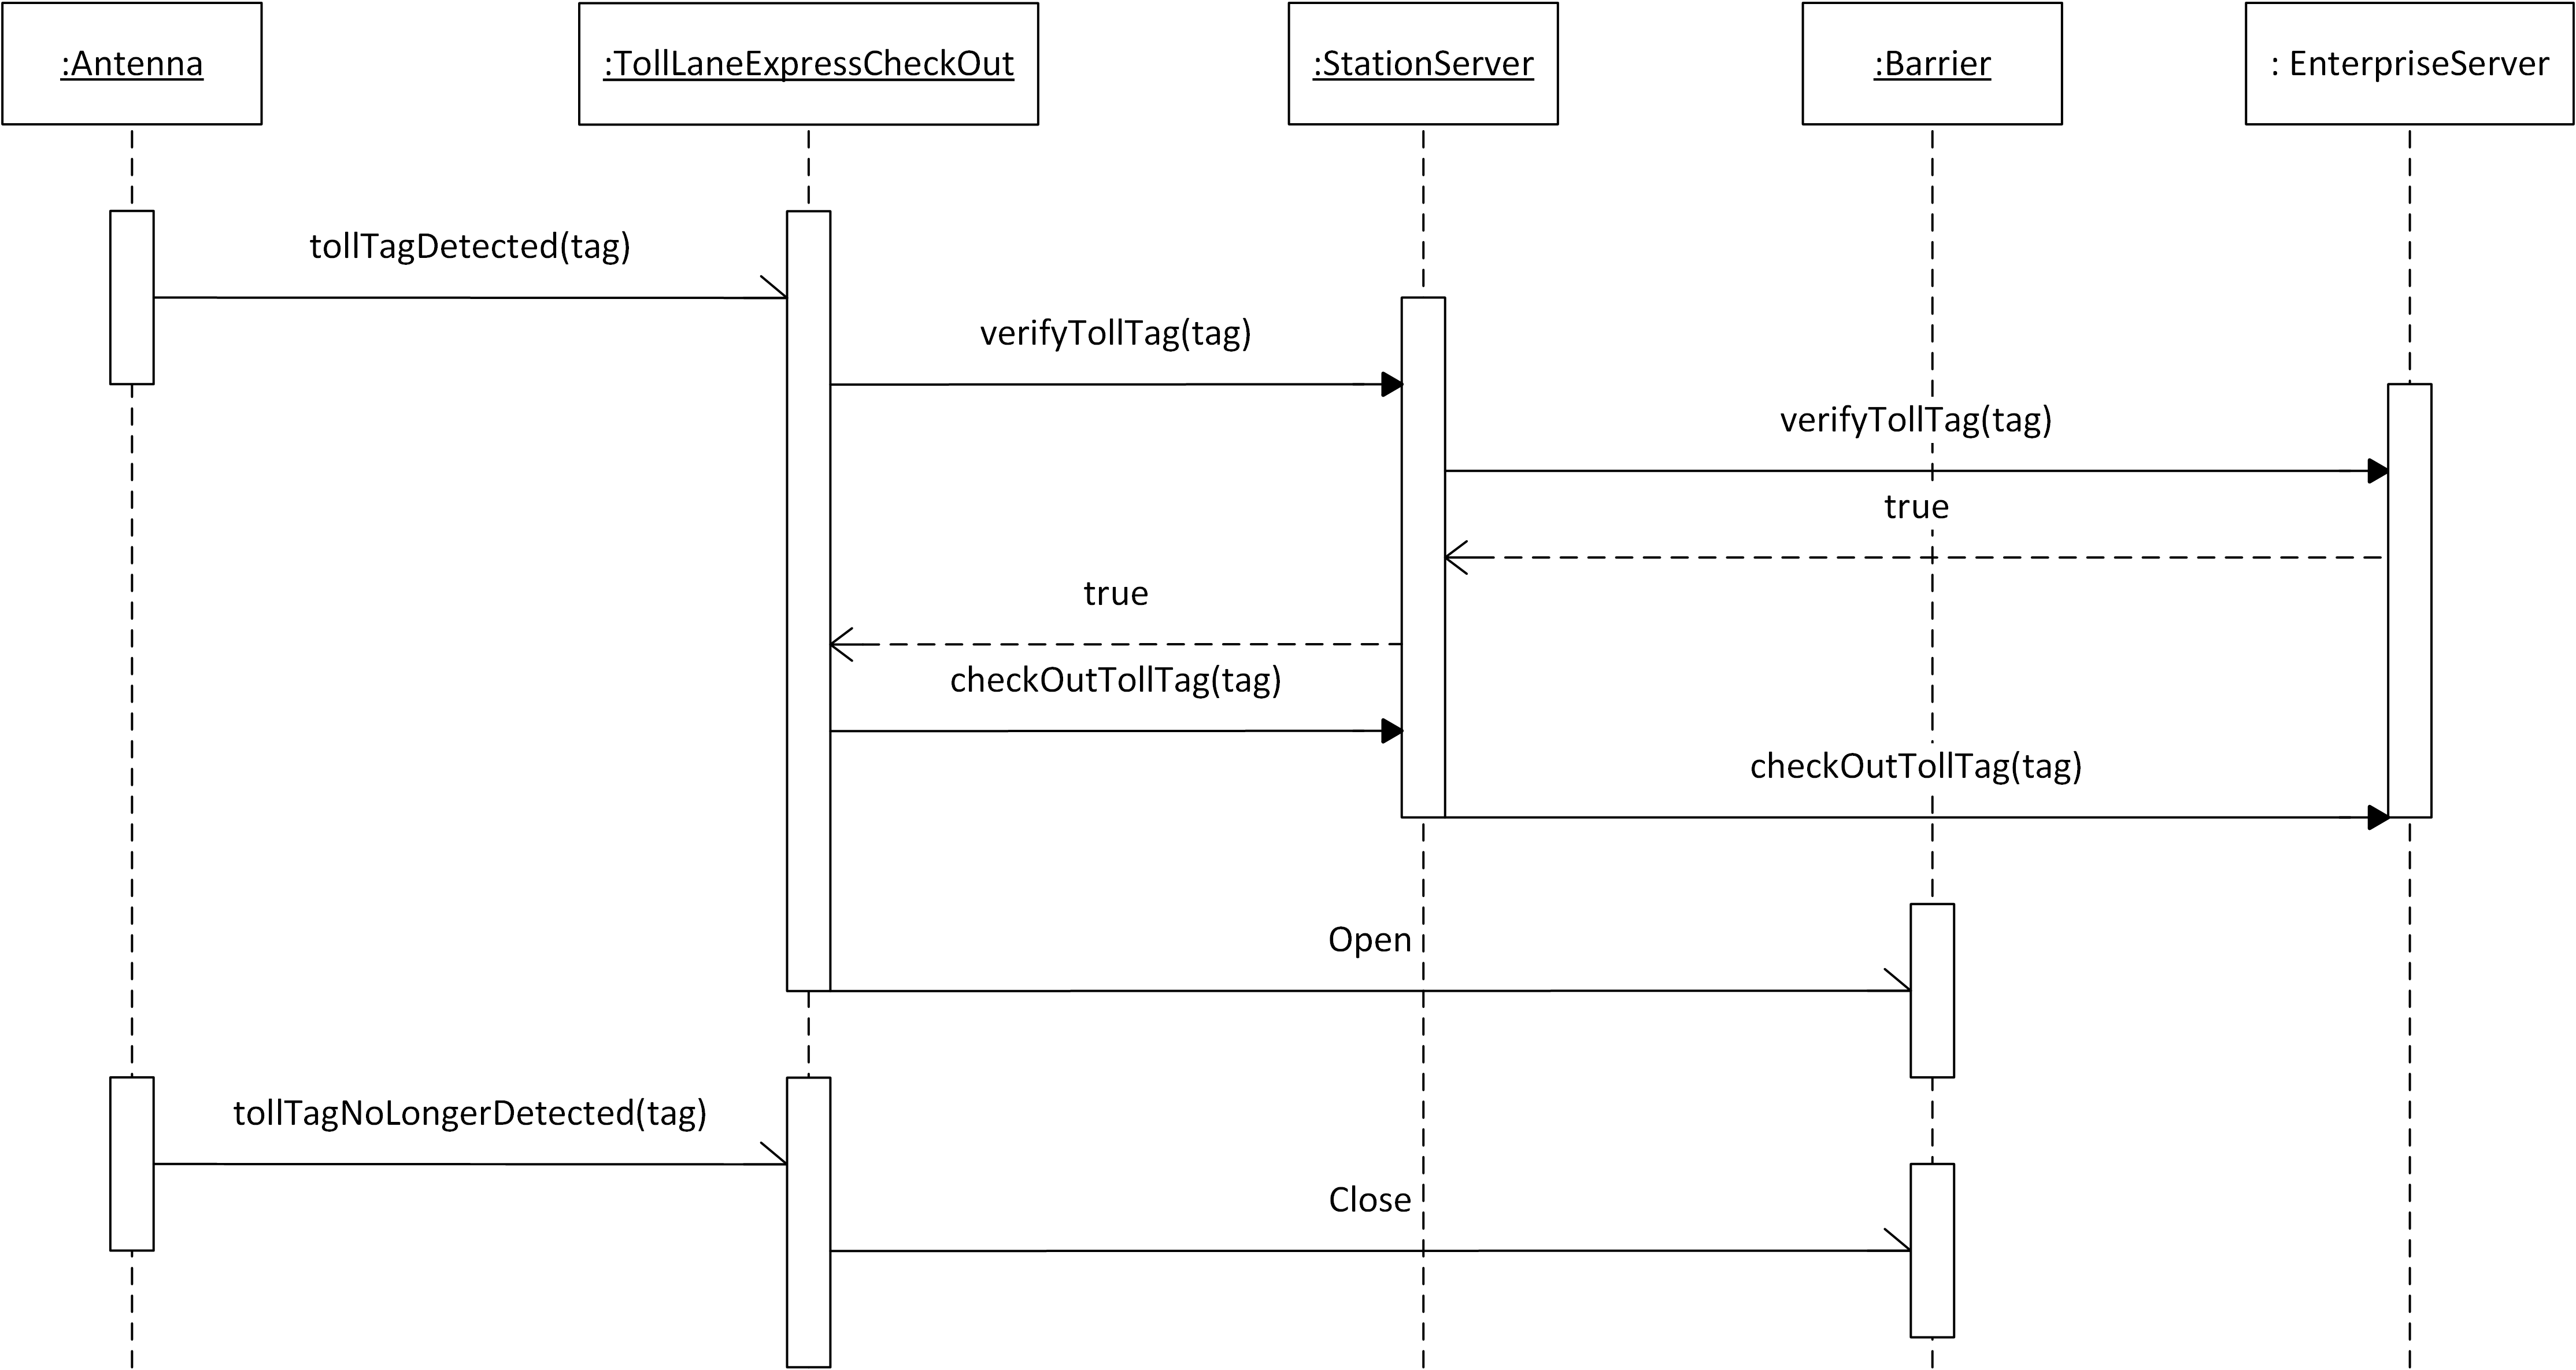
\includegraphics[width=1.4\columnwidth]{\lyxdot \lyxdot /report/img/sequence_diagrams/sequence_diagram_toll_tag_check_out}

\caption{Sequence diagram of toll tag check out}
\label{fig:seq_check_out_toll_tag}


\end{figure}

\begin{enumerate}
\item The customer drives up to the barrier, and awaits check-out.

\begin{enumerate}
\item The lane detects the customer's toll tag through the antenna by receiving
a tollTagDetected message.
\end{enumerate}
\item The system checks out the customer

\begin{enumerate}
\item The lane then checks out the tag by. 

\begin{enumerate}
\item It first sends verifyTollTag with the tag to the StationServer
\item The StationServer sends the same message to the EnterpriseServer
\item The EnterpriseServer then checks that the tag is checked in.
\item Once the EnterpriseServer has verified the tag it responds with ``true''
if the above condition held,
\item The StationServer sends the response back to the Express lane .
\item When the Express lane has received the response, if it was true it
will send a check out message which should now succeed.
\end{enumerate}
\end{enumerate}
\item The system opens the barrier.

\begin{enumerate}
\item Once the tag has been checked out, the Express lane will send the
message Open to the barrier, which will cause it to open
\end{enumerate}
\item The customer leaves the toll lane.

\begin{enumerate}
\item The lane will await the message tollTagNoLongerDetected from the antenna
which means the tag is no longer in range
\end{enumerate}
\item The system closes the barrier.

\begin{enumerate}
\item Once the Express has received tollTagNoLongerDetected, it will assume
it is safe to close the barrier. It will do that by sending a Close
message to the barrier.\end{enumerate}
\end{enumerate}

